\documentclass[12pt,a4paper]{article}
\usepackage[utf8]{inputenc}
\usepackage[T1]{fontenc}
\usepackage[spanish]{babel}
\usepackage{geometry}
\usepackage{hyperref}
\usepackage{graphicx}
\usepackage{listings}
\usepackage{xcolor}
\usepackage{booktabs}
\usepackage{tabularx}
\usepackage{caption}
\usepackage{float}
\usepackage{parskip}
\usepackage{enumitem}
\usepackage{titlesec}

\geometry{margin=2.5cm}

\addto\captionsspanish{\renewcommand{\tablename}{Tabla}}

\hypersetup{
  colorlinks=true,
  linkcolor=blue!60!black,
  urlcolor=blue!60!black,
  citecolor=blue!60!black
}

\definecolor{codegray}{rgb}{0.95,0.95,0.95}
\definecolor{codecomment}{rgb}{0.4,0.4,0.4}
\definecolor{codekeyword}{rgb}{0.0,0.3,0.7}
\definecolor{codestring}{rgb}{0.2,0.5,0.2}

\lstset{
  language=Java,
  backgroundcolor=\color{codegray},
  basicstyle=\ttfamily\small,
  keywordstyle=\color{codekeyword}\bfseries,
  commentstyle=\color{codecomment}\itshape,
  stringstyle=\color{codestring},
  numbers=left,
  numberstyle=\tiny\color{gray},
  numbersep=8pt,
  breaklines=true,
  showstringspaces=false,
  frame=single,
  framerule=0pt,
  xleftmargin=1em,
  xrightmargin=0.5em,
  captionpos=b,
  extendedchars=true,
  literate=
    {á}{{\'a}}1 {é}{{\'e}}1 {í}{{\'\i}}1 {ó}{{\'o}}1 {ú}{{\'u}}1
    {Á}{{\'A}}1 {É}{{\'E}}1 {Í}{{\'I}}1 {Ó}{{\'O}}1 {Ú}{{\'U}}1
    {ñ}{{\~n}}1 {Ñ}{{\~N}}1
}

\title{\textbf{Refactorización del sistema de excepciones en OpenMarkov}\\[0.5em]
\large Diseño, motivación e implementación}
\author{CISIAD --- UNED}
\date{Marzo 2026}

\begin{document}

\maketitle
\tableofcontents
\newpage

% ─────────────────────────────────────────────────────────────────────────────
\section{Introducción}
\label{sec:intro}

OpenMarkov es una herramienta de modelado con redes probabilísticas compuesta
por aproximadamente veinte módulos Maven y varios miles de clases Java.
Antes de la refactorización descrita en este documento, el proyecto definía
\textbf{61 clases de excepción propias}. La mayor parte de ellas eran excepciones
\emph{checked} (comprobadas), extendían \texttt{Exception} directamente y
carecían de cualquier clase base común dentro del dominio de la aplicación.

Esta situación generaba varios problemas prácticos: métodos de la interfaz gráfica
declaraban en su firma excepciones de bajo nivel que nunca podían manejar, el
compilador no podía verificar la exhaustividad de los bloques \texttt{catch} sobre
excepciones con múltiples variantes, y añadir una nueva acción en la GUI requería
copiar decenas de líneas de código de gestión de errores sin ningún valor
semántico.

Este informe documenta la refactorización completa del sistema de excepciones:
los problemas identificados, las decisiones de diseño tomadas y su justificación,
los cambios concretos aplicados al código y el impacto cuantitativo resultante.

% ─────────────────────────────────────────────────────────────────────────────
\section{Conceptos previos}
\label{sec:conceptos}

\subsection{Excepciones comprobadas y no comprobadas}
\label{sec:checked-unchecked}

Java distingue dos categorías de excepción:

\begin{description}[leftmargin=2em]
  \item[Comprobada (\textit{checked})] El compilador obliga al código que invoca
    un método a gestionar explícitamente la excepción: capturarla (\texttt{catch})
    o propagarla (\texttt{throws}). Heredan de \texttt{Exception} pero no de
    \texttt{RuntimeException}.
  \item[No comprobada (\textit{unchecked})] El compilador no impone ninguna
    obligación al llamador. Heredan de \texttt{RuntimeException}.
\end{description}

La elección tiene consecuencias arquitectónicas importantes. Una excepción
comprobada que ninguna capa intermedia puede resolver \emph{contamina} la firma
de todos los métodos por los que transita, forzando cláusulas \texttt{throws} que
no añaden información semántica. El principio generalmente aceptado es:

\begin{itemize}
  \item Usar \textbf{checked} cuando el llamador dispone de una acción correctiva
    concreta y razonable (abrir otro fichero, retirar la evidencia conflictiva).
  \item Usar \textbf{unchecked} cuando el error no es recuperable en la capa
    llamante o indica un problema de programación.
\end{itemize}

\subsection{Clases selladas (\textit{sealed classes})}
\label{sec:sealed}

Introducidas en Java~17, las clases selladas permiten declarar exactamente qué
subclases están permitidas:

\begin{lstlisting}[caption={Sintaxis de clase sellada}]
public abstract sealed class MiExcepcion extends RuntimeException
        permits MiExcepcion.CasoA, MiExcepcion.CasoB {

    public static final class CasoA extends MiExcepcion { ... }
    public static final class CasoB extends MiExcepcion { ... }
}
\end{lstlisting}

Las ventajas son:
\begin{itemize}
  \item El compilador garantiza exhaustividad en expresiones \texttt{switch}
    sobre el tipo.
  \item Es imposible añadir un subtipo accidentalmente desde otro módulo.
  \item Los subtipos posibles quedan documentados en el código con nombre propio
    y campos tipados, sin depender de comentarios o convenciones informales.
\end{itemize}

\subsection{Arquitectura en capas de OpenMarkov}
\label{sec:capas}

OpenMarkov sigue una arquitectura en capas donde cada módulo depende de los
inferiores pero no al revés:

\begin{center}
\begin{tabular}{cl}
\toprule
Nivel & Módulo \\
\midrule
4 & \texttt{org.openmarkov.gui} \\
3 & \texttt{org.openmarkov.inference}, \texttt{learning.*} \\
2 & \texttt{org.openmarkov.io.*} \\
1 & \texttt{org.openmarkov.core} \\
\bottomrule
\end{tabular}
\end{center}

Cuando un tipo concreto de una capa inferior aparece en la firma de un método de
una capa superior se produce una \textbf{fuga de abstracción}: la capa superior
queda acoplada a un detalle de implementación de la inferior, dificultando el
mantenimiento y los cambios futuros.

\subsection{Sistema de localización: \texttt{IBundledOpenMarkovException}}
\label{sec:i18n}

OpenMarkov incluye un sistema de mensajes de error localizados (i18n) basado en
ficheros \texttt{.properties}. La interfaz \texttt{IBundledOpenMarkovException}
actúa de puente entre las clases de excepción y dicho sistema:

\begin{lstlisting}[caption={Interfaz de localización de excepciones (extracto)}]
public interface IBundledOpenMarkovException extends IOpenMarkovException {

    default String getExceptionTitle() {
        // Deriva el título del nombre simple de la clase,
        // insertando espacios antes de las mayúsculas:
        // "WriterException" -> "Writer Exception"
        return ClassLocalizable.titleFromClassName(this.getClass());
    }

    default String getExceptionMessage() {
        // Busca la clave <NombreClase>.message en el .properties
        // correspondiente al módulo donde vive la excepción.
        return ClassLocalizable.messageFromClass(this.getClass());
    }

    static String toString(IBundledOpenMarkovException ex) {
        return ex.getExceptionTitle() + ": " + ex.getExceptionMessage();
    }
}
\end{lstlisting}

La convención del proyecto es que \textbf{toda excepción propia de OpenMarkov}
implemente esta interfaz, garantizando que los diálogos de error de la GUI
siempre dispongan de un título y un mensaje localizados sin código especial
en cada punto de captura.

% ─────────────────────────────────────────────────────────────────────────────
\section{Estado anterior: problemas identificados}
\label{sec:problemas}

\subsection{Ausencia de base común para excepciones de dominio}
\label{sec:prob-base}

Antes de la refactorización, las excepciones propias del proyecto extendían
directamente \texttt{Exception} o \texttt{RuntimeException} sin ningún tipo
intermedio propio. Esta situación impedía:

\begin{itemize}
  \item Capturar cualquier excepción de dominio de OpenMarkov en un único
    \texttt{catch} para tratamiento uniforme.
  \item Distinguir en tiempo de compilación entre una excepción de dominio y
    una excepción del sistema (\texttt{NullPointerException},
    \texttt{IOException}, etc.).
  \item Garantizar que todas las excepciones implementaran
    \texttt{IBundledOpenMarkovException}: sin clase base que la implementara,
    la presencia de la interfaz dependía de la disciplina del programador en
    cada clase individual.
\end{itemize}

\subsection{Excepciones comprobadas irrecuperables}
\label{sec:prob-checked}

Varios tipos de excepción estaban declarados como \emph{checked} a pesar de
representar condiciones de las que ninguna capa intermedia podía recuperarse.
El propio código lo reconocía con comentarios \texttt{TODO}:

\begin{itemize}
  \item \texttt{NonProjectablePotentialException}: «\textit{Almost every
    exception is wrapped into UnreacheableException or shown with JOptionPane}»
  \item \texttt{NotEvaluableNetworkException}: «\textit{Only caught to show a
    generic message}»
  \item \texttt{UnexpectedInferenceException}: «\textit{Catches are always
    wrapped with UnreacheableException}»
  \item \texttt{InvalidNetworkTypeException}: «\textit{Always wrapped in
    UnreacheableException}»
  \item \texttt{CannotNormalizePotentialException}: «\textit{Does this really
    happen in the GUI?}»
\end{itemize}

El efecto era una contaminación en cascada: \textbf{más de 40 cláusulas
\texttt{throws}} en firmas de métodos de la GUI, el motor de inferencia y los
módulos de aprendizaje, ninguna de las cuales añadía información semántica útil.
Métodos de Swing como \texttt{actionPerformed}, que por contrato del
\textit{framework} no deberían declarar excepciones, acumulaban cláusulas
\texttt{throws} que el compilador toleraba sin que tuvieran ningún significado
en ese contexto.

\subsection{Fuga de \texttt{SAXException} hasta la GUI}
\label{sec:prob-sax}

El método \texttt{MainPanelListenerAssistant.openNetwork()} declaraba
\texttt{throws SAXException}. \texttt{SAXException} pertenece a la biblioteca
estándar de procesado XML (JAXP/SAX) y es completamente ajena al dominio de
redes probabilísticas. Su presencia en la firma de un método de la capa de
presentación representa una fuga de abstracción: la GUI estaba acoplada a un
detalle de implementación del módulo de lectura de ficheros.

\subsection{Jerarquía plana con variantes implícitas}
\label{sec:prob-plana}

\texttt{NonProjectablePotentialException} agrupaba ocho causas de error distintas
sin ninguna estructura formal. Los bloques \texttt{catch} debían recurrir a
\texttt{instanceof} o a campos de texto para distinguirlas, lo que:

\begin{itemize}
  \item Requería que el programador conociera de memoria los subtipos informales.
  \item No era verificado por el compilador.
  \item Hacía que el código de manejo de errores fuera frágil ante la adición
    de nuevos casos.
\end{itemize}

\subsection{Bloques \texttt{try/catch} repetitivos en la GUI}
\label{sec:prob-try}

El método \texttt{actionPerformed} de \texttt{MainPanelListenerAssistant}
contenía aproximadamente \textbf{34 bloques} con la estructura:

\begin{lstlisting}[caption={Patrón repetitivo antes de la refactorización}]
try {
    accionConcreta();
} catch (ExcepcionComprobada1 ex) {
    throw new UnrecoverableException(ex);
} catch (ExcepcionComprobada2 ex) {
    throw new UnrecoverableException(ex);
}
\end{lstlisting}

Este código no añadía ninguna lógica: simplemente envolvía toda excepción
\emph{checked} en \texttt{UnrecoverableException}. Era ruido puro, propenso
a errores al añadir nuevas acciones y difícil de leer.

\subsection{Antipatrón \texttt{catch} $\to$ \texttt{null} en \texttt{FormatManager}}
\label{sec:prob-null}

El método de instanciación de plugins de \texttt{FormatManager} capturaba las
excepciones de reflexión y devolvía \texttt{null} sin registrar nada:

\begin{lstlisting}[caption={Antipatrón original en \texttt{FormatManager}}]
.map(readerClass -> {
    try {
        return readerClass.getDeclaredConstructor().newInstance();
    } catch (InstantiationException | NoSuchMethodException | ...) {
        return null;  // plugin mal configurado: fallo silencioso
    }
})
\end{lstlisting}

Un plugin mal configurado fallaba silenciosamente en este punto y provocaba
un \texttt{NullPointerException} sin traza útil en un punto posterior y
completamente distinto del origen del problema.

Además, el método \texttt{getProbNetReaderInstanceFor()} usaba
\texttt{.findFirst().get()} sobre el \texttt{Optional} resultante de la
búsqueda de lector. En ausencia de lector, este código lanzaba
\texttt{NoSuchElementException} en lugar de devolver \texttt{null}, convirtiendo
el \texttt{if (reader == null)} del llamador en código muerto e inalcanzable.

\subsection{Excepciones de navegación de casos de evidencia}
\label{sec:prob-nav}

\texttt{EvidenceManager} declaraba como \emph{checked}
\texttt{ThereIsNoPreviousEvidenceCaseException} y
\texttt{ThereIsNoNextEvidenceCaseException}. Sin embargo, el panel de controles
ya desactivaba los botones correspondientes antes de que pudieran provocar esas
condiciones. Las excepciones eran código muerto que se propagaba innecesariamente
a los módulos de inferencia y aprendizaje.

% ─────────────────────────────────────────────────────────────────────────────
\section{Diseño de la nueva jerarquía}
\label{sec:diseno}

\subsection{Criterio para la clasificación checked / unchecked}
\label{sec:criterio}

El criterio aplicado es semántico y se resume en la siguiente pregunta:

\begin{quote}
\textit{¿Existe en el llamador una acción correctiva concreta y razonable cuando
se produce este error?}
\end{quote}

\begin{itemize}
  \item Si la respuesta es \textbf{sí} (mostrar un diálogo y ofrecer abrir
    otro fichero, retirar la evidencia conflictiva, etc.): la excepción debe
    ser \textbf{checked}, para que el compilador obligue al llamador a
    considerar ese escenario.
  \item Si la respuesta es \textbf{no} (el llamador solo puede registrar el
    error y terminar, o la condición no debería ocurrir bajo un diseño correcto):
    la excepción debe ser \textbf{unchecked}, para no contaminar las firmas.
\end{itemize}

Aplicando este criterio, las cinco excepciones del §\,\ref{sec:prob-checked}
pasaron a ser \emph{unchecked}. El resto mantuvieron su carácter \emph{checked}.

\subsection{Clases base abstractas: \texttt{OpenMarkovRuntimeException} y
  \texttt{OpenMarkovException}}
\label{sec:bases}

Se crearon dos clases base abstractas simétricas para las dos categorías:

\begin{lstlisting}[caption={\texttt{OpenMarkovRuntimeException} — base \textit{unchecked}}]
public abstract class OpenMarkovRuntimeException extends RuntimeException
        implements IBundledOpenMarkovException {
    protected OpenMarkovRuntimeException() {}
    protected OpenMarkovRuntimeException(Throwable cause) { super(cause); }
}
\end{lstlisting}

\begin{lstlisting}[caption={\texttt{OpenMarkovException} — base \textit{checked}}]
public abstract class OpenMarkovException extends Exception
        implements IBundledOpenMarkovException {
    protected OpenMarkovException() {}
    protected OpenMarkovException(Throwable cause) { super(cause); }
    protected OpenMarkovException(String message) { super(message); }
    protected OpenMarkovException(String message, Throwable cause) {
        super(message, cause);
    }
}
\end{lstlisting}

\noindent\texttt{OpenMarkovException} define cuatro constructores (frente a dos
en \texttt{OpenMarkovRuntimeException}) porque las excepciones \emph{checked}
existentes que se migraban usaban también los constructores con \texttt{String}.

Al implementar \texttt{IBundledOpenMarkovException}, ambas clases base garantizan
que todas sus subclases hereden automáticamente
\texttt{getExceptionTitle()} y \texttt{getExceptionMessage()}, sin necesidad de
añadir la interfaz de forma individual en cada subclase.

\subsection{Agrupación semántica: \texttt{UserInputException}}
\label{sec:userinput}

Dentro de la jerarquía \emph{checked}, se identificó un grupo de excepciones con
una propiedad común: todas son consecuencia directa de lo que el usuario
proporciona al sistema, y la acción correctiva en todos los casos es mostrar un
mensaje informativo. Las excepciones del grupo son:

\begin{center}
\begin{tabular}{ll}
\toprule
Excepción & Causa \\
\midrule
\texttt{ParserException}               & Fichero abierto mal formado o versión no reconocida \\
\texttt{WriterException}               & Fallo al escribir el fichero de red \\
\texttt{IncompatibleEvidenceException} & Evidencia inconsistente con la red \\
\texttt{EmptyDatabaseException}        & Base de datos sin casos para aprendizaje \\
\texttt{ParsingSourceException}        & Expresión fuente con error sintáctico \\
\texttt{NoReaderForFileException}      & Ningún plugin puede leer el fichero indicado \\
\texttt{NoReaderForExtension}          & Sin lector para la extensión dada \\
\texttt{NoWriterForExtensionException} & Sin escritor para la extensión dada \\
\bottomrule
\end{tabular}
\end{center}

Se creó \texttt{UserInputException extends OpenMarkovException} como clase
intermedia abstracta y estas ocho excepciones pasaron a extenderla. La
motivación es doble:

\begin{enumerate}
  \item \textbf{Captura uniforme en la GUI.} El código de presentación puede
    escribir:
    \begin{lstlisting}[caption={Captura uniforme de errores de usuario}]
} catch (UserInputException ex) {
    showErrorDialog(ex.getExceptionTitle(),
                    ex.getExceptionMessage());
}
    \end{lstlisting}
    sin enumerar cada subtipo. La lista de subtipos puede crecer en el futuro
    sin modificar el código de la GUI.

  \item \textbf{Documentación estructural.} La pertenencia a
    \texttt{UserInputException} comunica a quien mantiene el código que el
    error es tratable a nivel de usuario, en contraposición a errores internos
    como \texttt{DoEditException} o \texttt{CostEffectivenessException}.
\end{enumerate}

\subsection{Excepciones \emph{checked} fuera de \texttt{UserInputException}}
\label{sec:otras-checked}

Las excepciones \emph{checked} que no se incluyeron en \texttt{UserInputException}
son aquellas cuyo tratamiento no consiste simplemente en mostrar un mensaje:

\begin{description}[leftmargin=2em]
  \item[\texttt{DoEditException} / \texttt{ConstraintViolatedException}]
    Señalizan fallos en operaciones de edición de la red (undo/redo) o violaciones
    de restricciones del modelo. Tienen puntos de captura específicos con lógica
    de tratamiento propia.
  \item[\texttt{CostEffectivenessException}] Indica configuraciones incorrectas
    en el análisis coste-efectividad, con validación específica.
  \item[\texttt{PotentialOperationException}] Fallo en operaciones matemáticas
    sobre potenciales, con tratamiento en el motor de inferencia.
  \item[Excepciones de intervalo] Restricciones de integridad matemática con
    validación en el modelo.
\end{description}

\subsection{Jerarquías selladas para excepciones con múltiples variantes}
\label{sec:sealed-design}

Para las excepciones con múltiples causas distintas se eligió el patrón de
\textbf{clase sellada con subclases internas estáticas}. El caso más
representativo es \texttt{NonProjectablePotentialException}:

\begin{lstlisting}[caption={Jerarquía sellada de
  \texttt{NonProjectablePotentialException} (extracto)}]
public abstract sealed class NonProjectablePotentialException
        extends OpenMarkovRuntimeException {

    public static final class SuperValueMustBeSumOrProduct
            extends NonProjectablePotentialException { ... }

    public static final class PotentialCannotBeConvertedToATable
            extends NonProjectablePotentialException { ... }

    public static final class MissingVariableInEvidence
            extends NonProjectablePotentialException {
        public MissingVariableInEvidence(Variable variable) { ... }
        public final Variable variable;
    }
    // ... cinco subtipos más
}
\end{lstlisting}

El mismo patrón se aplicó a \texttt{NotEvaluableNetworkException} (3~subtipos),
\texttt{InvalidNetworkTypeException} (2~subtipos),
\texttt{UnexpectedInferenceException} (1~subtipo), \texttt{WriterException}
(5~subtipos), \texttt{ParsingSourceException} (1~subtipo),
\texttt{CostEffectivenessException} (4~subtipos) y
\texttt{PotentialOperationException} (1~subtipo).

\subsection{Exclusión de \texttt{UnreachableException} y
  \texttt{UnrecoverableException}}
\label{sec:exclusion}

Estas dos excepciones tienen naturaleza distinta y fueron excluidas
deliberadamente de las jerarquías de dominio:

\begin{description}[leftmargin=2em]
  \item[\texttt{UnreachableException}] Señaliza código que, por diseño del
    sistema, nunca debería ejecutarse. Es equivalente a \texttt{assert false}:
    no es un error de dominio sino la violación de una invariante del programa.
    Incluirla en \texttt{OpenMarkovRuntimeException} habría confundido errores
    de dominio con errores de programación en los bloques \texttt{catch}.
  \item[\texttt{UnrecoverableException}] Es infraestructura de la GUI: envuelve
    cualquier excepción que alcanza el \textit{event dispatch thread} de Swing
    sin haber sido tratada. Su alcance es transversal, no específico del dominio.
\end{description}

\subsection{Preservación de nombres existentes}
\label{sec:nombres}

Una opción considerada fue renombrar excepciones para encajarlas en una nueva
taxonomía (por ejemplo, \texttt{NonProjectablePotentialException}
$\to$ \texttt{PotentialComputationException}). Esta opción se descartó porque:

\begin{itemize}
  \item Los nombres originales son vocabulario establecido entre los
    desarrolladores del proyecto y tienen significado semántico preciso en el
    dominio.
  \item El cambio de nombre habría requerido actualizar cientos de ficheros,
    introduciendo ruido en el historial de versiones sin beneficio funcional.
  \item La taxonomía deseada se expresa igualmente bien mediante herencia.
\end{itemize}

% ─────────────────────────────────────────────────────────────────────────────
\section{Cambios implementados}
\label{sec:cambios}

\subsection{Conversión a no comprobadas de cinco excepciones de dominio}
\label{sec:impl-unchecked}

Las cinco excepciones identificadas en §\,\ref{sec:prob-checked} se convirtieron
a \texttt{extends OpenMarkovRuntimeException}. Esto eliminó \textbf{más de
40~cláusulas \texttt{throws}} a través de 53~ficheros en cuatro módulos
(\texttt{core}, \texttt{gui}, \texttt{inference}, \texttt{learning.algorithm}).

\subsection{Jerarquías selladas}
\label{sec:impl-sealed}

\texttt{NonProjectablePotentialException} y otras seis excepciones se
convirtieron en clases selladas con subtipos internos tipados (véase
§\,\ref{sec:sealed-design}). Los bloques \texttt{catch} que anteriormente
recurrían a \texttt{instanceof} pueden ahora trabajar con tipos concretos
verificados en tiempo de compilación.

\subsection{Patrón \texttt{UIAction} en la GUI}
\label{sec:impl-uiaction}

Se introdujo la interfaz funcional \texttt{UIAction} y el método auxiliar
\texttt{executeUIAction} en \texttt{MainPanelListenerAssistant}:

\begin{lstlisting}[caption={Interfaz funcional \texttt{UIAction} y método auxiliar}]
@FunctionalInterface
private interface UIAction {
    void execute() throws Exception;
}

private void executeUIAction(UIAction action) {
    try {
        action.execute();
    } catch (RuntimeException ex) {
        throw ex;                       // deja pasar unchecked sin envolver
    } catch (Exception ex) {
        throw new UnrecoverableException(ex);
    }
}
\end{lstlisting}

Los 34~bloques \texttt{try/catch} repetitivos se reemplazaron por llamadas
de una sola línea:

\begin{lstlisting}[caption={Uso del patrón \texttt{UIAction} en \texttt{actionPerformed}}]
case ActionCommands.OPEN_NETWORK ->
    executeUIAction(() -> openNetwork());

case ActionCommands.COMPILE_NETWORK -> executeUIAction(() -> {
    compileNetwork();
    updateMenus();
});
\end{lstlisting}

Se dejaron fuera del patrón dos casos con lógica especial:
\texttt{CHANGE\_WORKING\_MODE} (tiene su propia lógica de confirmación de cambios
sin guardar) y \texttt{COST\_EFFECTIVENESS\_DETERMINISTIC} (lanza
\texttt{UnreachableException}, no una excepción comprobada).

\subsection{Encapsulación de \texttt{SAXException}}
\label{sec:impl-sax}

Se añadió un bloque \texttt{catch(SAXException)} en el interior de
\texttt{openNetwork()} que convierte la excepción en
\texttt{ParserException.BadlyStructuredFile} antes de que escape del método.
La firma de \texttt{openNetwork()} ya no menciona \texttt{SAXException} y la
GUI queda completamente aislada de la tecnología de \textit{parsing} XML.

\subsection{Eliminación de excepciones de navegación}
\label{sec:impl-nav}

Se eliminaron \texttt{ThereIsNoPreviousEvidenceCaseException} y
\texttt{ThereIsNoNextEvidenceCaseException}. Los bloques que las lanzaban se
sustituyeron por \texttt{UnreachableException}:

\begin{lstlisting}[caption={Guarda con \texttt{UnreachableException} en
  \texttt{goToPreviousEvidenceCase}}]
if (!(this.currentCase > 0)) {
    throw new UnreachableException(new IllegalStateException(
        "Go-to-previous button should have been disabled " +
        "when at first evidence case"));
}
\end{lstlisting}

\texttt{UnreachableException} comunica explícitamente a los futuros
mantenedores que esta rama es imposible bajo las invariantes actuales, a
diferencia de un comentario que puede quedar desfasado.

\subsection{Corrección del antipatrón en \texttt{FormatManager}}
\label{sec:impl-formatmanager}

Se realizaron dos correcciones:

\begin{enumerate}
  \item \textbf{Instanciación de plugins}: el bloque \texttt{catch} que
    devolvía \texttt{null} fue sustituido por
    \texttt{throw new UnreachableException(...)}, que incluye el nombre de la
    clase y la causa original.

  \item \textbf{Búsqueda de lector}: \texttt{.findFirst().get()} fue sustituido
    por \texttt{.findFirst().orElse(null)}, restaurando el comportamiento
    pretendido:

\begin{lstlisting}[caption={Corrección en \texttt{getProbNetReaderInstanceFor()}}]
// ANTES — lanza NoSuchElementException; el null-check es código muerto
return this.readerInstances.stream()
        .filter(plugin -> ...)
        .findFirst().get();

// DESPUÉS — retorna null; el llamador lanza NoReaderForFileException
return this.readerInstances.stream()
        .filter(plugin -> ...)
        .findFirst().orElse(null);
\end{lstlisting}
\end{enumerate}

\subsection{Creación de \texttt{OpenMarkovException} y migración de excepciones
  \emph{checked}}
\label{sec:impl-base}

Se creó la clase abstracta \texttt{OpenMarkovException} (véase §\,\ref{sec:bases})
y las excepciones \emph{checked} que extendían \texttt{Exception} directamente
se migraron a extenderla. El proceso afectó a \textbf{42~ficheros} en siete
módulos. La migración eliminó automáticamente las cláusulas
\texttt{implements IBundledOpenMarkovException} redundantes de cada una de ellas.

\subsection{Creación de \texttt{UserInputException}}
\label{sec:impl-userinput}

Se creó \texttt{UserInputException extends OpenMarkovException} y las ocho
excepciones descritas en §\,\ref{sec:userinput} pasaron a extenderla. El cambio
es \textbf{totalmente compatible hacia atrás}: cualquier código que capture
\texttt{OpenMarkovException} o un subtipo concreto continúa funcionando sin
modificaciones.

% ─────────────────────────────────────────────────────────────────────────────
\section{Jerarquía resultante}
\label{sec:jerarquia}

Las figuras~\ref{fig:checked} y~\ref{fig:unchecked} muestran la jerarquía de
excepciones tras la refactorización completa. Las clases sombreadas en verde
(\texttt{OpenMarkovException}, \texttt{UserInputException}) son nuevas. Las
sombreadas en azul (\texttt{OpenMarkovRuntimeException} y su rama) constituyen
la jerarquía \emph{unchecked}. Las sombreadas en rojo son clases de la
biblioteca estándar de Java.

\begin{figure}[H]
\centering
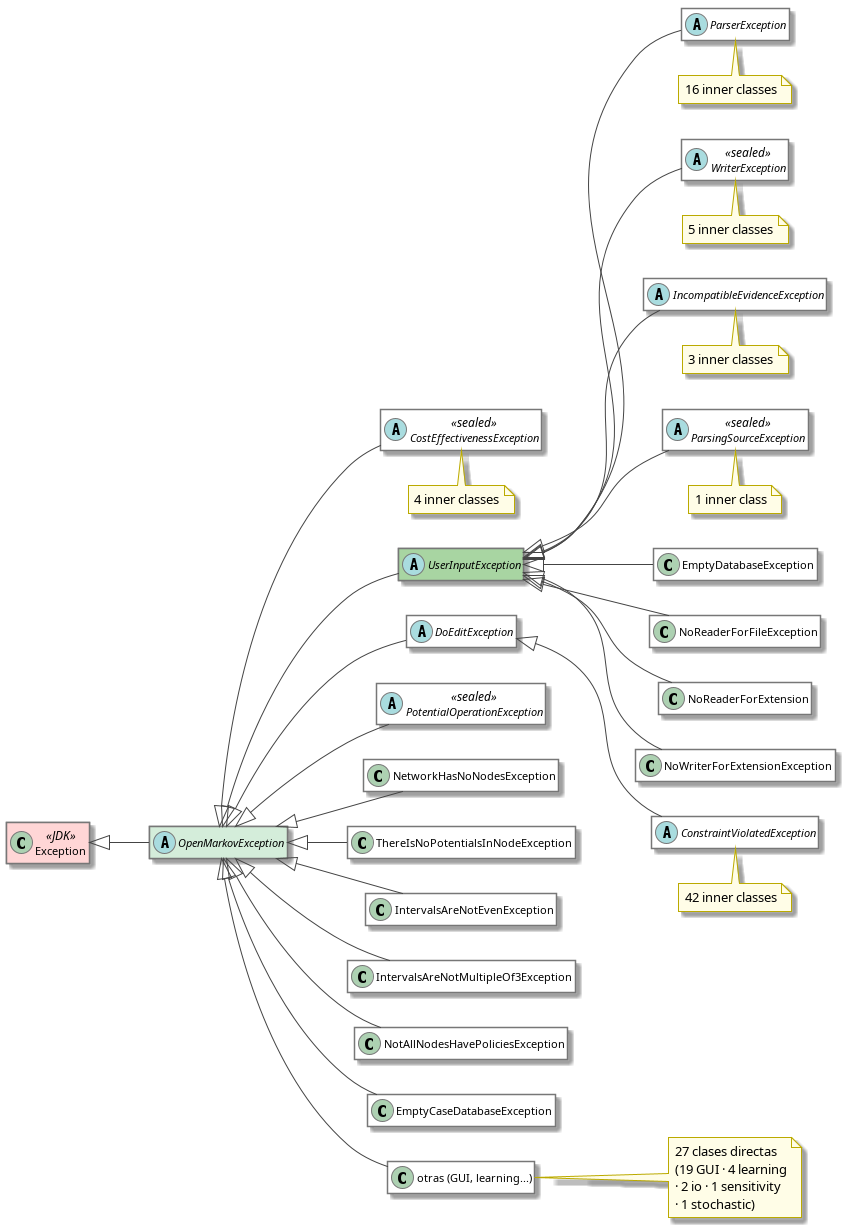
\includegraphics[width=0.90\linewidth]{hierarchy_checked.png}
\caption{Jerarquía \emph{checked} bajo \texttt{OpenMarkovException}.
  El número de \textit{inner classes} se indica en notas.
  Las clases en verde son nuevas.}
\label{fig:checked}
\end{figure}

\begin{figure}[H]
\centering
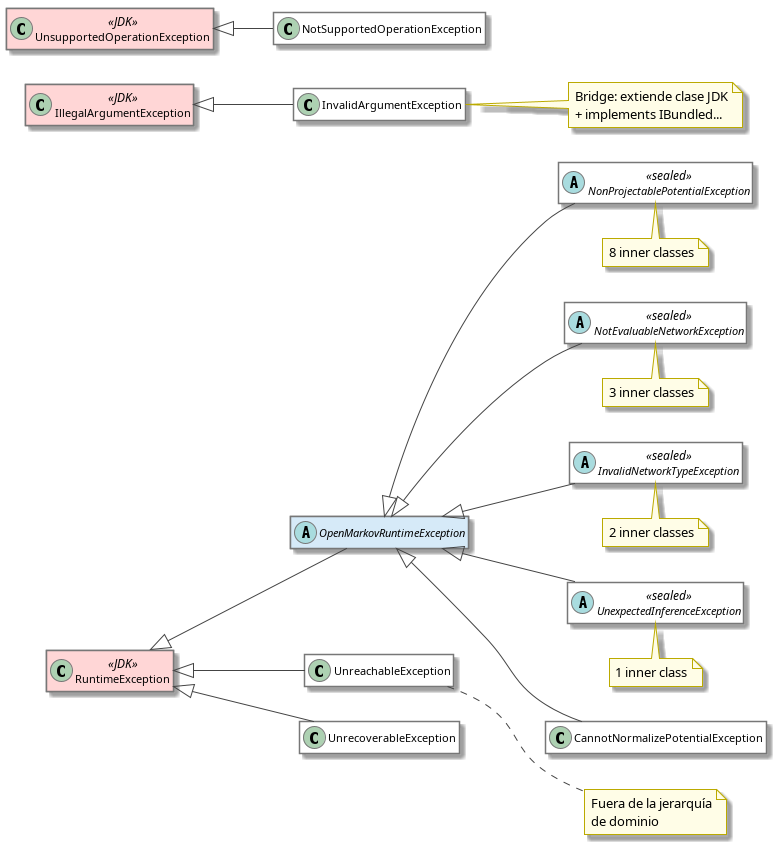
\includegraphics[width=0.80\linewidth]{hierarchy_unchecked.png}
\caption{Jerarquía \emph{unchecked} bajo \texttt{OpenMarkovRuntimeException}
  e infraestructura de gestión de errores.}
\label{fig:unchecked}
\end{figure}

% ─────────────────────────────────────────────────────────────────────────────
\section{Impacto cuantitativo}
\label{sec:impacto}

\begin{table}[H]
\centering
\begin{tabularx}{\textwidth}{p{6.2cm}rrX}
\toprule
Cambio & Ficheros & Elementos & Efecto \\
\midrule
Conversión de 5 excepciones a \textit{unchecked}
  & 53 & $-$40 \texttt{throws}
  & Elimina contaminación en cascada \\
Jerarquías selladas (7 excepciones)
  & 8 & $+$24 subtipos tipados
  & Exhaustividad en compilación \\
Patrón \texttt{UIAction} en GUI
  & 1 & $-$34 bloques \texttt{try/catch}
  & Elimina código repetitivo \\
Encapsulación de \texttt{SAXException}
  & 1 & $-$1 \texttt{throws SAXException}
  & Elimina fuga de abstracción \\
\texttt{OpenMarkovRuntimeException}
  & 6 & $+$1 base; $+$5 herencias
  & Base común \textit{unchecked} \\
Eliminación de excepciones de navegación
  & 3 & $-$2 clases
  & Elimina código muerto \\
Corrección \texttt{FormatManager}
  & 1 & 2 bugs corregidos
  & Fallos dejan de ser silenciosos \\
\texttt{OpenMarkovException}
  & 1 & $+$1 base \textit{checked}
  & Base común \textit{checked} \\
Migración de 42 excepciones \textit{checked}
  & 42 & $-$42 \texttt{implements} redundantes
  & Coherencia de jerarquía \\
\texttt{UserInputException}
  & 9 & $+$1 intermedia; $+$8 herencias
  & Agrupación semántica \\
\midrule
\textbf{Total}
  & \textbf{$\sim$125}
  & \textbf{net $\approx -$115}
  & \\
\bottomrule
\end{tabularx}
\caption{Resumen cuantitativo de la refactorización}
\label{tab:impacto}
\end{table}

% ─────────────────────────────────────────────────────────────────────────────
\section{Conclusiones}
\label{sec:conclusiones}

La refactorización del sistema de excepciones de OpenMarkov produjo las siguientes
mejoras concretas:

\begin{description}[leftmargin=2em]
  \item[Legibilidad] Los métodos expresan su lógica sin distracciones de manejo
    de errores que no aportan información. La eliminación de 40~cláusulas
    \texttt{throws} en cascada es el ejemplo más visible.

  \item[Coherencia del modelo de errores] Todas las excepciones de dominio
    comparten una raíz común (\texttt{OpenMarkovException} o
    \texttt{OpenMarkovRuntimeException}) que garantiza la implementación de
    \texttt{IBundledOpenMarkovException} sin depender de la disciplina individual
    del programador.

  \item[Seguridad estática] Las jerarquías selladas permiten que el compilador
    detecte bloques \texttt{switch} no exhaustivos sobre las variantes de las
    excepciones más complejas.

  \item[Expresividad de intención] \texttt{UserInputException} comunica
    estructuralmente qué errores son orientados al usuario y cuáles son internos.
    \texttt{UnreachableException} documenta en el código mismo que una rama es
    imposible según las invariantes del sistema, de forma más fiable que un
    comentario.

  \item[Mantenibilidad] Añadir una nueva acción en \texttt{actionPerformed} ya
    no requiere recordar el patrón \texttt{try/catch} repetitivo. Añadir una nueva
    excepción orientada al usuario solo requiere extender
    \texttt{UserInputException}.

  \item[Separación de capas] La GUI ya no conoce \texttt{SAXException} ni ningún
    otro detalle de implementación de la capa de E/S.

  \item[Diagnóstico de errores] Los fallos en la instanciación de plugins de
    \texttt{FormatManager} incluyen ahora el nombre de la clase problemática y la
    causa original en lugar de fallar silenciosamente varios pasos después.
\end{description}

Todos los tests existentes pasan tras la refactorización, lo que proporciona
confianza en que no se han introducido regresiones en el comportamiento observable.

\end{document}
